% Gemini theme
% https://github.com/anishathalye/gemini

\documentclass[final]{beamer}

% ====================
% Packages
% ====================

\usepackage{amsmath}
\usepackage{mathdots}
\usepackage[T1]{fontenc}
\usepackage{lmodern}
\usepackage[size=a0,orientation=portrait,scale=1.3]{beamerposter}
\usetheme{gemini}
\usecolortheme{uq}
\usepackage{graphicx}
\usepackage{tikz}
\usetikzlibrary{shapes.geometric, arrows, positioning, fit, bayesnet}
\usepackage{natbib}
\usepackage{url}
\usepackage{listings}

\lstset{% general command to set parameter(s)
basicstyle=\small\sffamily,
language=haskell,
moredelim=**[is][\color{gray}]{~}{~},
morekeywords={P},
literate={+}{{$+$}}1 {/}{{$/$}}1 {*}{{$*$}}1
           {=}{{$=\ $}}1 %{/=}{{$\neg$}}1
           %{>}{{$>$}}1 {<}{{$<$}}1 %{\\}{{$\lambda$}}1
           %{++}{{$+\!\!\!+\;$}}1 %{::}{{$:\!\!\!:$}}1
           %{$}{{\texttt{\$}\hspace{0.5em}}}1
           {==}{{$=\!=\;$}}2
           %{\\\\}{{\char`\\\char`\\}}1
           {->}{{$\rightarrow$}}2 {>=}{{$\geq$}}2 {<-}{{$\leftarrow$}}2
           {<=}{{$\leq$}}2 {=>}{{$\Rightarrow$}}2
           {\ .\ }{{$\;\circ$}}2 {(.)}{{($\ \circ$)}}2
           {<<}{{$\ll$}}2 {>>}{{$\gg\;$}}2 
           {>>=}{{$>\!\!>\!\!=$}}2
           {=<<}{{$=\!<\!\!<$}}2
           {|}{{$\mid$}}1
           {undefined}{{$\bot$}}1
           % {not\ }{{$\neg$}}1
           {`elem`}{{$\in$}}1
           {forall}{{$\forall$}}1
           {'}{{${}^\prime$}}1
}

% ====================
% Lengths
% ====================

% If you have N columns, choose \sepwidth and \colwidth such that
% (N+1)*\sepwidth + N*\colwidth = \paperwidth
\newlength{\sepwidth}
\newlength{\colwidth}
\setlength{\sepwidth}{0.025\paperwidth}
\setlength{\colwidth}{0.4625\paperwidth}

\newcommand{\separatorcolumn}{\begin{column}{\sepwidth}\end{column}}

% ====================
% Title
% ====================

\title{Reversible Jump Probabilistic Programming}

\author{David A Roberts \and Marcus Gallagher \and Thomas Taimre}

%\institute[shortinst]{The University of Queensland, Australia}

\institute{\url{https://davidar.github.io/stochaskell}}

% ====================
% Body
% ====================

\begin{document}

\addtobeamertemplate{headline}{}
{
  \begin{tikzpicture}[remember picture,overlay]
    \node [anchor=north east, xshift=-\sepwidth, yshift=-6.5cm] at (current page.north east) {
\includegraphics[height=3cm]{images/uq-logo-white}};
  \end{tikzpicture}
}

\tikzstyle{prog} = [line width=0.5mm, rectangle, fill=green!20, draw=green!50!black, minimum width=6.5cm, minimum height=2.5cm]
\tikzstyle{math} = [line width=0.5mm, rectangle, fill=blue!20, draw=blue!50!black, minimum width=6.5cm, minimum height=2.5cm]
\tikzstyle {op} = [circle, inner sep=0, minimum size=2.5cm]
\tikzstyle{container} = [line width=0.5mm, draw=black!50]
\tikzstyle{arrow} = [line width=1mm, ->, >=latex]
\tikzstyle{elab} = [font=\small]

\begin{frame}[t]
  \begin{columns}[t]
    \separatorcolumn

    \begin{column}{\colwidth}
      \begin{center}
        \usebeamerfont{headline}\usebeamercolor[fg]{heading}\mdseries\Large
        Automatically generating Reversible Jump Markov chain Monte Carlo samplers from user-provided target and proposal probabilistic programs
      \end{center}

      \bigskip

      \begin{block}{Reversible Jump Markov chain Monte Carlo (RJMCMC)}
        \begin{itemize}
          \item As with Metropolis--Hastings (M--H), RJMCMC generates candidate states via a proposal distribution and accepts/rejects according to an \textcolor{purple}{\bfseries acceptance ratio}:
                \begin{center}
                  \begin{tabular*}{0.75\linewidth}{c @{\extracolsep{\fill}} c}
                    \textcolor{purple}{\bfseries M--H} & \textcolor{purple}{\bfseries RJMCMC} \\
                    $\displaystyle\alpha_{x \to x^*} = \frac{f(x^*)q(x|x^*)}{f(x)q(x^*|x)}$ &
                    $\displaystyle\alpha_{x \to x^*} = \frac{f(x^*)g^*(u^*)}{f(x)g(u)}
                      \textcolor{purple}{\left|\frac{\partial(x^*,u^*)}{\partial(x,u)}\right|}$ \\
                  \end{tabular*}
                \end{center}
          \item Application to probabilistic programming requires automatic derivation of $\alpha$
          \item \textcolor{purple}{\bfseries Jacobian} depends on structure of problem-specific proposal distribution
        \end{itemize}
      \end{block}

      \begin{alertblock}{Automatic derivation of RJMCMC inference program}
        \centering

        \begin{tikzpicture}[x=2.5cm,y=2.5cm]

          \node (prior0) {prior};
          \node (prior1) [prog, below=0.1 of prior0] {$v \sim p$};
          \node (prior2) [prog, below=0.25 of prior1] {$x = t(v)$};
          \node (invt) [math, below=1.75 of prior2] {$v = t^{-1}(x)$};
          \node (jact) [math, right=0.25 of invt, minimum width=4.375cm] {$\frac{\partial x}{\partial v}$};
          \node (fx) [math, below=0.25 of invt.south west, anchor=north west, minimum width=11.5cm]
          {$f(x) = p(t^{-1}(x)) / \left|\frac{\partial x}{\partial v}\right|$};
          \node (fxratio) [math, below=1.66 of fx] {$\displaystyle\frac{f(x^*)}{f(x)}$};
          \node (guratio) [math, right=0.25 of fxratio] {$\displaystyle\frac{g^*(u^*)}{g(u)}$};

          \node (prop1) [prog, right=5 of prior1] {$u \sim g$};
          \node (prop2) [prog, below=0.25 of prop1] {$x^* = h(u;x)$};
          \node (prop0) [above=0.1 of prop1] {proposal$_x$};
          \node (invh) [math, below=1.75 of prop2] {$u^* = h^{-1}(x;x^*)$};
          \node (dinvh) [math, below=1.5 of invh] {$\frac{\partial h^{-1}(x;x^*)}{\partial (x,x^*)}$};
          \node (dh) [math, right=0.25 of dinvh] {$\frac{\partial h(u;x)}{\partial (x,u)}$};
          \node (jac) [math, right=0.25 of guratio]
          {$\begin{vmatrix}
                \frac{\partial h(u;x)}{\partial x} & \frac{\partial h(u;x)}{\partial u}                                              \\
                \frac{\partial h^{-1}(x;x^*)}{\partial x}
                + \frac{\partial h^{-1}(x;x^*)}{\partial x^{*}}\frac{\partial h(u;x)}{\partial x}
                                                   & \frac{\partial h^{-1}(x;x^*)}{\partial x^{*}}\frac{\partial h(u;x)}{\partial u}
              \end{vmatrix}$};

          \node (prior) [container, fit={(prior0) (prior1) (prior2)}] {};
          \node (prop) [container, fit={(prop0) (prop1) (prop2)}] {};

          \node (alpha) [math, below=0.5 of guratio] {$\alpha_{x \to x^*}$};
          \node (rjmc) [prog, below=0.5 of alpha, align=left, minimum width=3.5, minimum height=1.25]
          {$x^* \sim \text{proposal}_x$ \\ accept w.p.\ $\min(1,\alpha_{x \to x^*})$};
          \node [left=0.1 of rjmc, align=right] {RJMC\\transition};
          \node (ir) [prog, right=1.9 of rjmc, minimum width=3cm] {IR};
          \node (cpp) [prog, right=2 of ir, minimum width=4cm] {C++};

          \draw [arrow] (prior2) -- node[elab, anchor=south, rotate=90] {auto inv.} (invt);
          \draw [arrow] (prior2) -| node[elab, anchor=south east, rotate=90] {auto diff.} (jact);
          \draw [arrow] (jact) -- (fx);
          \draw [arrow] (invt) -- (fx);
          \draw [arrow] (prior1.west) -- +(-0.4,0) |- (fx);
          \draw [arrow] (fx) -- (fxratio);

          \draw [arrow] (prop1) -| (guratio);
          \draw [arrow] (prop2) -- node[elab, anchor=south, rotate=90] {auto inv.} (invh);
          \draw [arrow] (invh) -- node[elab, anchor=south, rotate=90] {auto diff.} (dinvh);
          \draw [arrow] (prop2) -| node[elab, anchor=south east, rotate=90] {auto diff.} (dh);
          \draw [arrow] (dinvh) -- (jac);
          \draw [arrow] (dh) -- (jac);

          \draw [arrow] (fxratio) to[out=270, in=180] (alpha);
          \draw [arrow] (guratio) -- (alpha);
          \draw [arrow] (jac) to[out=225, in=0] (alpha);
          \draw [arrow] (alpha) -- (rjmc);
          \draw [arrow] ([yshift=2.5cm]prop.east) to[out=-30, in=90] ([xshift=0.75cm]jac.south east) to[out=270,in=30] (rjmc);
          \draw [arrow] (rjmc) -- node[elab, anchor=south] {code} node[elab, anchor=north] {optimiser} (ir);
          \draw [arrow] (ir)   -- node[elab, anchor=south] {code} node[elab, anchor=north] {generator} (cpp);

        \end{tikzpicture}

      \end{alertblock}

      \begin{block}{Automatic transformation inversion}
        \begin{itemize}
          \item Recursively apply rewrite rules to invert outermost operation:
                \begin{equation*}
                  \begin{split}
                    x^* \, \mathrm{insertAt}(i,\exp(u^*)) & = x
                  \end{split}
                  \quad\underset{\mathrm{insertAt}^{-1}}\Rightarrow\quad
                  \begin{split}
                    i & = \mathrm{find}_j(x^*_j \neq x_j) \\
                    \exp(u^*) & = x_i \quad\underset{\exp^{-1}}\Rightarrow\quad u^* = \log x_i
                  \end{split}
                \end{equation*}

          \item Solving \textcolor{purple}{\bfseries case expressions}, i.e. $h(u^*;x^*) = x$ where
                \begin{align*}
                  h(u^*;x^*) & = \begin{cases}
                    e_1 & \text{if }e_0 = 1           \\
                    e_2 & \phantom{\text{if }}e_0 = 2 \\
                        & \vdots                      \\
                    e_n & \phantom{\text{if }}e_0 = n \\
                  \end{cases}
                \end{align*}

                \begin{itemize}
                  \item First solve component expressions, e.g.:

                        \bigskip
                        \begin{center}
                          \setlength\tabcolsep{1em}
                          \begin{tabular}{c|c|ll}
                            $j$ & solve $e_0 = j$ & \multicolumn{2}{c}{solve $e_j = x$}                    \\
                            \hline
                            $1$ & $k = 0$         & $x^*_1 = x_1 + 1$                   & $u^*_1 = \alpha$ \\
                            $2$ & $k = 1$         & $x^*_1 = x_1 - 1$                   & $u^*_1 = \beta $ \\
                            $3$ & $k = 2$         & $x^*_2 = x_2$                       & $u^*_2 = \gamma$ \\
                            $4$ & $k = 3$         & $x^*_3 = x_3$                       & $u^*_2 = \delta$ \\
                          \end{tabular}
                        \end{center}
                        \bigskip

                  \item Combine to form final solutions:
                        \begin{align*}
                          \begin{split}
                            k & =\begin{cases}
                              0 & \text{if }x^*_1 = x_1 + 1           \\
                              1 & \phantom{\text{if }}x^*_1 = x_1 - 1 \\
                              2 & \phantom{\text{if }}x^*_2 = x_2     \\
                              3 & \phantom{\text{if }}x^*_3 = x_3
                            \end{cases}
                          \end{split}
                          \begin{split}
                            u_{1}^{*} & =\begin{cases}
                              \alpha & \text{if }k = 0           \\
                              \beta  & \phantom{\text{if }}k = 1
                            \end{cases} \\
                            u_{2}^{*} & =\begin{cases}
                              \gamma & \text{if }k = 2           \\
                              \delta & \phantom{\text{if }}k = 3
                            \end{cases}
                          \end{split}
                        \end{align*}
                \end{itemize}
        \end{itemize}

        \heading{Notation}
        {\footnotesize
          \begin{tabular}{rlrlrlrl}
            $f$ & target density    & $x$ & (current) state & $x^*$     & candidate state            & $q$ & M--H proposal density     \\
            $g$ & auxiliary density & $u$ & auxiliary r.v.  & $g^*,u^*$ & reverse proposal auxiliary & $h$ & reversible transformation
          \end{tabular}
        }

      \end{block}

    \end{column}

    \separatorcolumn

    \begin{column}{\colwidth}

      \begin{block}{Stochaskell intermediate representation}
        \begin{center}
          \begin{tikzpicture}[node distance=3.5cm]
            \node[math,op] (xi) {!};
            \node[math,op,below of=xi] (xj) {!};
            \node[minimum size=0,above left=0.25cm and 0.25cm of xi] (i) {$i$};
            \node[minimum size=0,below left=0.25cm and 0.25cm of xj,node distance=1cm] (j) {$j$};
            \node[math,op,right of=xi] (xij) {$-$};
            \node[math,op,right of=xij] (sq) {$\times$};
            \node[math,op,right of=sq] (div) {$/$};
            \node[above left=0.25cm and 0.25cm of div,minimum size=0,node distance=1cm] (two) {$2$};
            \node[math,op,right of=div] (neg) {$-$};
            \node[above left=0.25cm and 0.25cm of neg,minimum size=0,node distance=1cm] (zero) {$0$};
            \node[math,op,right of=neg] (exp) {$\exp$};

            \node[math,op,right of=xj] (eq) {$=$};
            \node[math,op,ellipse,right=2.5 of eq] (if) {ifThenElse};
            \node[below left  = 0.25cm and 0 of if,minimum size=0,node distance=1cm] (eta) {$10^{-6}$};
            \node[below right = 0.25cm and 0 of if,minimum size=0,node distance=1cm] (eta0) {$0$};
            \node[math,op, below of=exp,double] (elem) {$+$};

            \begin{scope}[minimum size=0]
              \plate {cov} {(i)(j)(xi)(xj)(zero)(two)(eta)(elem)} {$i=1,\ldots n,\quad j=1,\ldots n$};
            \end{scope}

            \node[prog,left=1cm of cov,yshift=0.5cm] (x) {$x \sim \mathsf{orderedSample}_\mathsf{uniform}$};
            \node[below left=-1.1cm and 1cm of x,minimum size=0,node distance=1.5cm] (lb) {$0$};
            \node[above left=-1.1cm and 1cm of x,minimum size=0,node distance=1.5cm] (ub) {$5$};
            \node[prog,above of=x] (n) {$n \sim \mathsf{poisson}$};
            \node[left=1 of n,minimum size=0] (five) {$5$};
            \node[prog,below of=x,double] (g) {$g \sim \mathsf{normal}$};
            \node[left=1 of g,minimum size=0] (zerov) {$\mathbf{0}$};

            \draw [arrow] (i) -- (xi);
            \draw [arrow] (j) -- (xj);
            \draw [arrow] (x) -- (xi);
            \draw [arrow] (x) -- (xj);
            \draw [arrow] (xi) -- (xij);
            \draw [arrow] (xj) -- (xij);
            \draw [arrow] (xij) to[bend right=10] (sq);
            \draw [arrow] (xij) to[bend left=10] (sq);
            \draw [arrow] (sq) -- (div);
            \draw [arrow] (two) -- (div);
            \draw [arrow] (zero) -- (neg);
            \draw [arrow] (div) -- (neg);
            \draw [arrow] (neg) -- (exp);

            \draw [arrow] (xi) -- (eq);
            \draw [arrow] (xj) -- (eq);
            \draw [arrow] (eq) -- (if);
            \draw [arrow] (eta) -- (if);
            \draw [arrow] (eta0) -- (if);
            \draw [arrow] (if) -- (elem);
            \draw [arrow] (exp) -- (elem);

            \draw [arrow] (five) -- (n);
            \draw [arrow] (n) -- (cov);
            \draw [arrow] (n) -- (x);
            \draw [arrow] (lb) -- (x);
            \draw [arrow] (ub) -- (x);
            \draw [arrow] (zerov) -- (g);
            \draw [arrow] (cov) -- (g);
          \end{tikzpicture}
        \end{center}

        \heading{Inversion by recursive graph rewriting}

        \begin{center}
          \begin{tikzpicture}
            \node (a1) [prog] {$a \sim \mathsf{normal}$};
            \node (b1) [prog, below=0.5 of a1] {$b \sim \mathsf{normal}$};
            \node (t1) [math,op, right=2 of a1] {$\times$};
            \node (p1) [math,op, right=2 of b1] {$+$};
            \node (c1) [above left=0.5 and 0.5 of t1, minimum size=0, inner sep=0] {$2$};
            \node (x1) [right=2 of t1] {$x$};
            \node (y1) [right=2 of p1] {$y$};

            \draw [arrow, dotted] (a1) -- (t1);
            \draw [arrow] (c1) -- (t1);
            \draw [arrow, dotted] (t1) -- (x1);
            \draw [arrow, dotted] (a1.south east) -- (p1);
            \draw [arrow, dotted] (b1) -- (p1);
            \draw [arrow, dotted] (p1) -- (y1);

            \node (a2) [prog, below=2 of b1] {$a = x / 2$};
            \node (b2) [prog, below=0.5 of a2] {$b \sim \mathsf{normal}$};
            \node (t2) [math,op, right=2 of a2] {$\div$};
            \node (p2) [math,op, right=2 of b2] {$+$};
            \node (c2) [above left=0.5 and 0.5 of t2, minimum size=0, inner sep=0] {$2$};
            \node (x2) [right=2 of t2] {$x$};
            \node (y2) [right=2 of p2] {$y$};

            \draw [arrow] (t2) -- (a2);
            \draw [arrow] (c2) -- (t2);
            \draw [arrow] (x2) -- (t2);
            \draw [arrow] (a2.south east) -- (p2);
            \draw [arrow, dotted] (b2) -- (p2);
            \draw [arrow, dotted] (p2) -- (y2);

            \node (a3) [prog, right=2 of x2] {$a = x / 2$};
            \node (b3) [prog, below=0.5 of a3] {$b = y - a$};
            \node (t3) [math,op, right=2 of a3] {$\div$};
            \node (p3) [math,op, right=2 of b3] {$-$};
            \node (c3) [above left=0.5 and 0.5 of t3, minimum size=0, inner sep=0] {$2$};
            \node (x3) [right=2 of t3] {$x$};
            \node (y3) [right=2 of p3] {$y$};

            \draw [arrow] (t3) -- (a3);
            \draw [arrow] (c3) -- (t3);
            \draw [arrow] (x3) -- (t3);
            \draw [arrow] (a3.south east) -- (p3);
            \draw [arrow] (p3) -- (b3);
            \draw [arrow] (y3) -- (p3);

            \node [right=2 of x1, yshift=-1cm, inner sep=0] {\lstinputlisting{solve.hs}};
          \end{tikzpicture}
        \end{center}
      \end{block}

      \begin{block}{Stochaskell example: coal mining disasters \citep{green_reversible_1995}}

        \heading{User-supplied code (high-level)}
        \begin{minipage}[t]{.49\linewidth}
          \lstinputlisting{coal1.hs}
        \end{minipage}
        \begin{minipage}[t]{.5\linewidth}
          \lstinputlisting{coal2.hs}
        \end{minipage}
        \lstinputlisting{coal3.hs}

        \definecolor{plotblue}{rgb}{0.25, 0.25, 1}
        \definecolor{plotgreen}{rgb}{0.25, 0.625, 0.25}
        \definecolor{plotred}{rgb}{1, 0.25, 0.25}

        \heading{Output}
        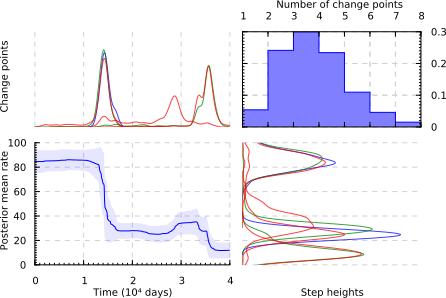
\includegraphics[width=\linewidth]{images/coal} \\
        {\footnotesize Marginal plots provide density estimates for elements of $\mathbf{s}$ (change point locations) and $\mathbf{g}$ (step heights) for $n = \textcolor{plotblue}{\mathbf{1}}, \textcolor{plotgreen}{\mathbf{2}}, \textcolor{plotred}{\mathbf{3}}$}

      \end{block}

      \begin{block}{Future work}
        \begin{itemize}
          \item Improve efficiency of generated code
                \begin{itemize}
                  \item General-purpose code optimisation
                  \item Algebraic expression simplification
                \end{itemize}
          \item Support inversion of more general transformations than
                $$h(\mathbf{u};x)=(h_1(u_1;x),h_2(u_1,u_2;x),\ldots,h_n(\mathbf{u};x))$$
        \end{itemize}
      \end{block}

      \heading{References}
      \nocite{*}
      {\footnotesize\bibliographystyle{apalike}\bibliography{poster}}

    \end{column}

    \separatorcolumn
  \end{columns}
\end{frame}

\end{document}
